%************************************************
\chapter{\texttt{aRNAque}: An evolutionary algorithm for inverse folding inspired by Lévy flights.}\label{ch:arnaque}

Among the optimisation techniques presented in the previous chapter, the EA has demonstrated good statistical performance and provide an interesting framework for studying the evolutionary dynamics of biological systems. Since the genetic algorithm (or more generally evolutionary algorithm) was proposed by John Holland \cite{holland1992adaptation} in the early 1970s, it has emerged as a popular search heuristic and found application in many disciplines that deal with complex landscape optimization problems. Most of the evolutionary algorithms and stochastic search techniques are  guided by local (or one-point mutations) mutations. Although a local search can efficiently discover optima in a simple landscape, more complex landscapes pose challenges to the design of evolutionary algorithms that rely solely on local search. This is especially true on a landscape with high neutrality  where local search may be inefficient or risk getting stuck on a plateau (or local optimum). To avoid this pitfall, we propose here a new tool called \texttt{aRNAque} which implements a mutation scheme inspired by Lévy flights (called Lévy mutation) and supports pseudoknotted RNA target structures.

Lévy flights are random walks with a Lévy (or any heavy-tailed) step size distribution. The concept originates in the work of Mandelbrot on the fluctuation of commodities prices in the 1960s \cite{mandelbrot1972certain}, but has since found many more physical applications \cite{shlesinger1995levy}. The term "Lévy flight" was also coined by Mandelbrot, who used one specific distribution of step sizes (the Lévy distribution, named after the french mathematician Paul Lévy). Lévy flights also play a key role in the context of animal foraging, perhaps because they provide an optimal balance between exploration and exploitation \cite{viswanathan2008levy,kamaruzaman2013levy}. For a recent review of applications of Lévy flights in biology from the molecular to the ecological scale \cite{reynolds2018current}.

Similar to a Lévy flight, a Lévy mutation scheme allows simultaneous search at all scales over the landscape. New mutations most often produce nearby sequences (one-point mutations), but occasionally generate mutant sequences which are far away in genotype space (macro-mutations). In this work, the distribution of the number of point mutations at every step is taken to follow a Zipf distribution. 

In the coming sections, we provide a detailed description of \text{aRNAque} algorithm and the experimental result when compared to existing tools.

	
\section{Material and methods}

\subsection{Inverse folding evolutionary algorithm (EA)}
In general, an evolutionary search algorithm on any fitness landscape consists of three main parts, which in the context of RNA inverse folding are as follows: %(Figure \ref{Fig:model}):
\begin{itemize}
	\item Initialization: generating a random initial population of RNA sequences compatible with the given target secondary structure.
	\item Evaluation and selection: evaluating a population of RNA sequences consists of two steps: 1) fold each sequence into a secondary structure and assign it a weight based on its similarity to the target structure. 2) select a weighted random sample with replacement from the current population to generate a new population. A detailed description of the objective function used in \texttt{aRNAque} is provided in the next section. 
	\item Mutation (or move) operation: define a set of rules or steps used to produce new sequences from the selected or initial ones. This component is elaborated further in the next subsection.
	
\end{itemize}
%\begin{figure}[H]
%    \centering
%    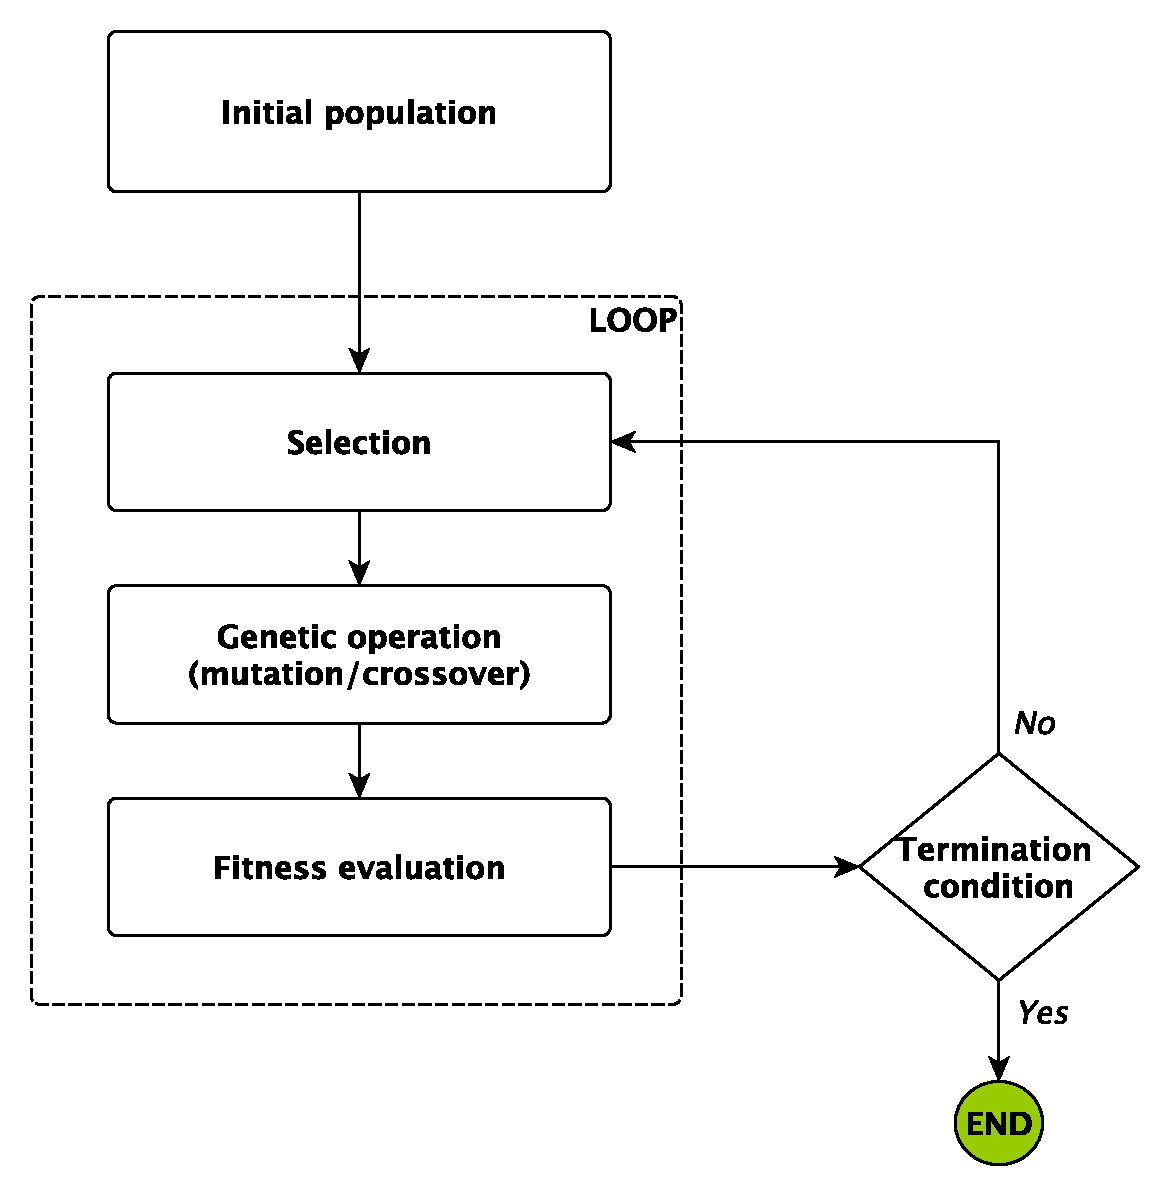
\includegraphics[width=0.5\textwidth]{figures/EA_draw.pdf}
%    \caption{Evolutionary algorithm flow diagram}
%    \label{Fig:model}
%\end{figure}


\subsection{\texttt{aRNAque}'s mutation operator}

For a given target RNA secondary structure $\sigma*$ of length $L$, the space of potential solutions to the inverse folding problem is $S=\{A,C,G,U\}^L$.
An evolutionary algorithm explores the space $S$ through its move (or mutation) operator. to explore exclusively the search space of compatible sequences (sequences with canonical base pairs at the corresponding open and closed bracket positions) with $\sigma^*$ , we introduce a mutation step that depends on the nucleotide and canonical base pair probability distribution.

Let~\(\mathcal{N}= \big \{ A, U, C, G \big \}\)~be the set of nucleotides weighted respectively by the probabilities:
\begin{equation*}
P_{\mathcal{N}} = \big \{ P_A, P_U, P_C, P_G \big\}
\end{equation*}
and~\(\mathcal{C} = \big \{ AU, UA, CG, GC, UG, GU\big \}\)~be the set of canonical base pairs weighted respectively by the probabilities:
\begin{equation*}
P_{\mathcal{C}} = \big \{P_{AU}, P_{UA},P_{CG},P_{GC},P_{UG},P_{UG} \big \} 
\end{equation*}
where
\begin{equation*}
\sum P_{\mathcal{N}} = 1, \sum P_{\mathcal{C}}  = 1 
\end{equation*}
and
\begin{equation*}
P_{AU} = P_{UA}, P_{UG} =P_{GU}, P_{CG} = P_{GC}
\end{equation*}
Therefore, our evolutionary algorithm relies on the flexibility of the mutation parameters $P_{\mathcal{N}}, P_{\mathcal{C}}$. These parameters allow the user to explicitly set the GC-content constraints , which allow the control of the nucleotide distribution during the design process.


\begin{figure*}[ht]
	\includegraphics[width=1.0 \linewidth]{../res/images/arnaque/fig1.pdf}
	\caption{Binomial \emph{vs.} Zipf distributions. (A) Samplings Binomial and Zipf distributions for the best binomial mutation rate $\mu^*$ (respectively $c^*$ for the best Zipf exponent parameter). Both distributions have a mean of $8.7$ point mutations for a sequence of length $88$ nucleotides. (B) Tuning of binomial mutation rate parameter. For each $\mu \in [0,1]$ with a step size of $0.005$ and the pseudoknotted target \texttt{PKB00342} of length $88$, $50$ sequences were designed using \texttt{aRNAque}. (B) shows the median generations and the success percentage \emph{vs.} the mutation rate ($\mu$). The best mutation rate is $\mu^*=0.085$ (with a median number of generation $93.5$ and a success rate of $92\%$). (C) Tuning of Levy exponent. Similar to (B), for each $c \in [0,7]$ with a step size of $0.1$ and for the same pseudoknotted target structure, $100$ sequences were designed using \texttt{aRNAque}. It shows the median generations and the percentage of success \emph{vs.} the exponent parameter ($c$). The Zipf exponent distribution that produced the highest success rate and the minimum number of generations is $c^*=1.4$.}\label{Fig:histomut}. 
\end{figure*}
 We examined the binomial and Zipf distributions:

\begin{itemize}
	\item Binomial mutation: here $U$ has a binomial distribution: 
	$$
	P(U=n)= \binom{L}{n} \mu^n (1-\mu)^{L-n}
	$$
	for some $0 \leq \mu \leq 1$, such that $u=\mu \cdot L$. We can think of this mutation mode arising from each nucleotide of an RNA sequence independently undergoing a point mutation with probability $\mu$, i.e. $\mu$ is the per-nucleotide or point mutation rate. 
	
	\item Lévy mutation: $U$ has a Zipf distribution given by: 
	$$
	P(U=n)= \frac{1/n^c}{ \sum_{k=1}^{L}{1/k^c}}
	$$
	where $c>0$ is the value of the exponent characterizing the distribution.
\end{itemize}

Figure \ref{Fig:histomut} shows the distribution of the number of point mutations on a sequence of length $88$ nucleotides for both mutation schemes. Both distributions have the same mean, and the difference between the two distributions is more perceptible on their tails. 

In the rest of this work, a local mutation will refer to a binomial mutation with parameter $\mu \approx 1/L$.

We present the mutation algorithm in Algorithm \ref{Algo:Lévy}.

\begin{algorithm}
	\tcc{$P'=\{S'_1\dots S'_n\}$: the mutated population\; 
		$P= \{S_1\dots S_n\}$: a list of $n$ RNA sequences to mutate\;
		$P_{C}=\{w_{AU},w_{GU},w_{GC}\}$: a vector containing the weights associated with each canonical base pairs\;
		$P_{N}=\{w_{A},w_{U},w_{C}, w_{G}\}$: a vector containing the weights associated with each nucleotide\;
		$\mathcal{D}$: a given probability distribution (Lévy or Binomial) with parameter $p$ and $L$ where $L$ is the length of the target RNA structure}
	\KwInput{$P$, $\mathcal{D}(p, L)$, $P_{C}$,  $P_{N}$}
	\KwOutput{$P'$} 
	$ \{B_i\} \sim \mathcal{D}(p,L)$, where $i\in \{1,2,\dots,n\}$ \tcp*{Draw $n$ random numbers that follows a given distribution $\mathcal{D} (p,L)$ (Lévy or Binomial). $B_i$ is the number base pairs to mutate}
	$\{U_i\} \sim \mathcal{D}(p,L)$, where $i\in \{1,2,\dots,n\}$ \tcp*{Draw $n$ random numbers that follows the same distribution as $B_i$ (Lévy or Binomial). $U_i$ is the number non base pair positions to mutate}
	
	\For{ $i \in \{1, 2, \dots, n\}$ }{
		$S'\leftarrow P_i$ \tcp*{Assign the sequence $S_i \in P$ to $S'$ }
		\For{ $j \in \{1,2,...U_i\}$}{
			$r \in \{1,2,\dots, L\} \sim \mathcal{U}$ \tcp*{select uniformly a random position in the RNA sequence $S'$}
			$n_j \in \{A,U,C,G\} \sim P_N$ \tcp*{select a random nucleotide $n_j$ with respect to $P_N$} 
			$S'_r \leftarrow n_{j}$ \tcp*{replace the nucleotide at position $j$ in the RNA sequence $S'$ with $n_j$}
		}
		\For{ $j \in \{1,2,...B_i\}$}{
			$k_j \in \{AU,UA,CG,GC,GU,UG\} \sim P_C$ \tcp*{select a random base pair $k_{i}$ with respect to $P_C$}
			$b \in \{(b_1,b_2)_i\} \sim \mathcal{U}$ \tcp*{select uniformly a random pair of base pair positions}
			$S'_b \leftarrow k_{j}$ \tcp*{replace respectively the nucleotides at the base pair position $b_i \in b$ by $k \in k_j$}
			
		}
		$P' \gets P'\cup S'$ \tcp*{Add $S'$ to the list $P'$}
	}
	\caption{Mutation algorithm}\label{Algo:Lévy}
\end{algorithm}
%In addition to the two main features mentioned above, we also provide a web-server integrating an enriching interface to compare and analyse the designed sequences.

%%%%%%%%%%%%%%%%%%%%%%%%%%%%%%%%%%%%%%%%%%%%%%
%%                                          %%
%% Backmatter begins here                   %%
%%                                          %%
%%%%%%%%%%%%%%%%%%%%%%%%%%%%%%%%%%%%%%%%%%%%%%

\subsection{\texttt{aRNAque}'s objection functions}
Our EA reaches its performance through the minimization of three objective functions:

\begin{itemize}
	%\tightlist
	\item
	Hamming distance from the target structure:~since the main goal of the inverse folding problem is to find sequences that fold into a given target secondary structure~\(\sigma*\), the simple fitness measurement~\(f\) of an RNA sequence~\(\phi\)~can be defined as follows:
\end{itemize}

\begin{equation}
\label{fitness}
f(\phi, \sigma*) = \frac{1}{1 + d(s^{MFE}(\phi) , \sigma*)}
\end{equation}

where~\(d(\cdot,\cdot)\)~is the hamming distance on the structure space (structures are in dot and bracket representation).

\begin{itemize}
	%\tightlist
	\item
	Normalized Energy Distance (NED): the difference between
	the energy of a given sequence~\(\phi\)~evaluated to fold
	into a target structure~\(\sigma*\)~and the minimum free energy
	of the sequence in its structural ensemble~\(\Gamma\).~ The value is normalized over all the sequences in a given population $P$.  
\end{itemize}

\begin{equation}
\label{ned}
NED(\phi, \sigma*) = [1-\Delta E_{norm}(\phi, \sigma*)]^p \text{   } \forall p>1
\end{equation}
where,
\begin{equation}
\Delta E_{norm}(\phi, \sigma*) = \frac{\Delta E(\phi, \sigma*) }{\sum_{\phi \in P}{\Delta E(\phi, \sigma*)}}
\end{equation}
and,
\begin{equation}
\Delta E(\phi, \sigma*) = E(\phi, \sigma*) - \arg \min_{s \in \Gamma} E(\phi, s)
\end{equation}

\begin{itemize}
	%\tightlist
	\item
	Ensemble defect (ED) \cite{zadeh2011nucleic}: Here, we use the ED as a second objective function for refinement after having at least one sequence that folds into the target in the current population. It is defined in Equation \ref{ed}.
\end{itemize}


To minimize the $NED$ (Eq. (\ref{ned})) and the hamming distance (or maximize the fitness (Eq. (\ref{fitness})) of a population of RNA sequences, instead of combining both measurements to form a multi-objective function, we use them separately at a different level of our EA. We use the $NED$ as a selection weight for the sequences that will be mutated, and the hamming distance is used as a weight to elite ten best sequences that will always move to the next generation. Therefore the selection method we use is the \textit{fitness proportionate selection}, also known as roulette wheel selection \cite{lipowski2012roulette}. Once we have at least one sequence that folds into the given target in the current population (for the successful case), we walk through its neutral network by minimizing the ensemble defect function (Eq. (\ref{ed})). This ED minimization is simply performed by replacing the $NED$ objective function by the $ED$ function the EA (Step 4).

\subsection{\texttt{aRNAque}'s EA}

For a given population size $N$ and a target structure $\sigma*$ of length $l$, an initial population $P$ is generated randomly as follows: 

\begin{enumerate}
	\item Select randomly $l$ nucleotides in $N_{ucl.}$
	
	\item Identify the base pair position $(i,j)$ in the random sequence, select randomly a base pair in the set of canonical base pairs $C_{bp}$ and fix the first nucleotide of the selected canonical base pair at the position $i$ and the second at position $j$.
	
	\item  Repeat 2. for all base pair positions in the target structure
	
	\item Repeat 1. 2. and 3 $N-$times.
\end{enumerate}
Let \(T\) be the maximum number of generations and \(F_t\) the set of all sequences found at a given time ~\(t\). After the initial population of RNA sequences is generated, our algorithm is performed as follows:
\vspace{0.05cm}

\(\texttt{While}\) \((t<T)\)~or~\( |F_t| <n_f\)
\(\texttt{do}\) :

\begin{itemize}
	%\tightlist
	\item Evaluate the fitness (Eq. (\ref{fitness})) of every sequence \(s \in P\)
	\item
	Add to \(F_t\)~all the sequences with fitness equal to $1$
	\item
	Choose~\(10\)~best sequences of~\(P\)~based
	on their fitness (Eq. (\ref{fitness})) values and add them to \(P'\)~.
	\item
	Sample~\(N\) sequences with respect to their \textit{NED} (Eq. (\ref{ned})) values and store them in~\(S\).
	\item
	\(\texttt{For}\) each RNA sequence ~\(s \in S\):~
\end{itemize}

\begin{quote}
	\begin{enumerate}
		%\tightlist
		\item
		\(s'\) = \(\texttt{copy(s)}\)~
		\item
		Select a random nucleotide~\(r_n
		\)
		in~\(N_{ucl.}\)~respect to the
		probabilities~\(P_{nucl.}\)~
		\item
		\(s'[i] = r_n\), where~\(i\)~is a random integer
		chosen uniformly from \(0\)~to \(l-1\)~
		\item
		Select a random base paire~\(b_p
		\) in~\(C_{bp}\)~
		respect to the probalities~\(P_{can.}
		\)
		\item
		\(s'[i] \leftarrow b_p[0]\)~and \(s'[j] \leftarrow b_p[1]\), where \((i,j)\)
		is a random tuple of integers chosen uniformly from the set of base
		pair positions.~
		\item
		Add~\(s'\) in \(P'\)~
	\end{enumerate}
\end{quote}

\begin{itemize}
	%\tightlist
	\item
	\(P \leftarrow P'\)
	\item
	\(t \leftarrow t + 1\)
\end{itemize}

\subsection{Parameter analysis and benchmark data}
Here we analyse mutation parameters and compare local and Lévy mutation modes. 

\subsubsection{Benchmark data used}
The \texttt{PseudoBase++} is a set of $266$ pseudoknotted RNA structures used to benchmark \texttt{Modena}. It was initially $342$ RNA secondary structures, but because of the redundancy and the non-canonical base pairs  $76$ structures were excluded. To group the dataset with respect to the pseudoknot motifs (Figure \ref{Fig:pk_type}), we used the test data from \texttt{antaRNA}'s paper. The test data contains $249$ grouped into four categories: $209$ hairpin pseudoknots (H), $29$ bulge pseudoknots (B), $8$ complex hairpin pseudoknots (cH) and $3$ kissing hairpin pseudoknots (K). Out of the $266$ structures, only $185$ (with $150$ H-type, $3$ K-type, $25$ B-type and $7$ cH-type) structures were included in the test data. So for that reason, we have used only $185$ target structures for the pseudoknot motif performance comparison and the $266$ structures for the different target lengths performance comparison.

The \(\texttt{Eterna100}\) dataset \cite{Eterna} is available in two versions and both contain a set of \(100\) target structures extracted from the \texttt{EteRNA} puzzle game and classified by their degree of difficulty. The \texttt{Eterna100-V1} was initially designed using \texttt{ViennaRNA} 1.8.5, which relies on Turner1999 energy parameters \cite{Turn1999}. Out of the $100$ target secondary structures, $19$ turned out to be unsolvable using the version of \texttt{ViennaRNA} $2.4.14$ (which relays on the Turner2004 \cite{mathews2004incorporating}). Subsequently, an \texttt{Eterna100-V2} \cite{Eterna} was released in which the $19$ targets were slightly modified to be solvable using \texttt{ViennaRNA} $2.4.14$ and any version that supports the Turner2004 energy parameters. The main difference between the two dataset relay on the energy parameters used to generate the data.

The \texttt{non-EteRNA} dataset: a set of \(63\) experimentally synthesized targets that Garcia-Martin et al. \cite{garcia2013rnaifold} recently used to benchmark a set of ten inverse folding algorithms, which from our knowledge, is the most recent and comprehensive benchmark of current state-of-the-art methods. The dataset is collected from \(3\) sources: the first dataset called \(\textbf{dataset A}\) which contains \(29\) targets collected from RFAM and also used in \cite{esmaili2015erd,taneda2011modena} and the second called \(\textbf{dataset B}\) is a collection of \(24\) targets used in \cite{esmaili2015erd} and added to that the \(10\) structures used in \cite{shi2018sentrna}.

\subsection{Benchmark protocol}
\subsubsection*{Folding tools}
Two tools for pseudoknotted RNA folding are considered in this work: \texttt{HotKnots} and \texttt{IPknot}. For pseudoknot-free RNA folding, we used \texttt{RNAfold}.
 For the mutation parameter and GC-content analysis presented in our work, we used \texttt{IPknot}, and both \texttt{HotKnots} and \texttt{IPknot} for \texttt{PseudobBse++} benchmarks. To be able to use \texttt{HotKnots} in \texttt{aRNAque} without copying \texttt{aRNAque} in the bin directory of \texttt{Hotknots}, we have performed some modifications on \texttt{Hotknots} source code. Details on the modifications are provided in the supplementary material SI 6. Furthermore, we considered \texttt{pkiss}, a well known tool for K-type pseudoknot prediction, but since the \texttt{PseudoBase++} dataset contains just $4$ K-type pseudoknotted structures and \texttt{pKiss} has higher time complexity ($O(n^6)$), we did not find it efficient for the benchmark we performed.
\subsubsection*{Mutation parameters tuning}
One of the main challenges for an evolutionary algorithm is to find optimum parameters such as mutation rate, population size and selection function.
We used $80$ pseudoknotted targets with lengths from $25$ to $181$ nucleotides for the mutation parameter analysis. We set the maximum number of generations $T$ to $200$ and the population size $n$ to $100$. The stopping criteria are two: 1) the number of generations ($t$) is equal to the max number of generations ($T$) or 2)the minimum hamming (or base pair) distance of the best RNA sequence solution to the target is $0$. The best mutation parameters ($c^*$ for Levy and $\mu^*$ for Binomial) are those that have the lowest median number of generations. The best mutation parameters obtained for both binomial and Lévy mutation modes are used to benchmark and compare the results on the entire datasets of RNA structures.
\subsubsection*{Benchmark on the \texttt{PseudoBase++} dataset}
Four benchmarks are performed on the pseudoknotted dataset: 1) mutation parameter analysis, 2) the GC-content and diversity analysis, 3) Local search versus Lévy search, 4) \texttt{aRNAque} (Lévy search) versus \texttt{antaRNA}. For the \texttt{aRNAque} (Binomial and Lévy) case, the four benchmarks share the same number maximum number of generations ($T=200$), population size ($n=100$), stopping criteria ($t=T$ or min fitness equals $0$).
For the \texttt{antaRNA} benchmark, the maximum number of iterations was set to $1200$, and a slight modification was made to allow the support of the folding tool $\texttt{HotKnots}$ (See SI 6).  
For booth tools and each benchmark,  $20$ runs were launched independently in parallel on a computer with the same resources, resulting in $20$ designed sequences per pseudoknotted target structure. To measure the performance of each tool, each designed sequence $s$ is folded into a secondary structure $\sigma$ and the similarities between $\sigma$ and $\sigma^*$ are computed using the base pair distance. 
For the GC-content benchmark, four GC-content values are considered, $\{0.25, 0.5, 0.75,1\}$ and the setting of each tool remains the same.
\subsubsection*{Benchmark on the \texttt{Eterna100} dataset}
We performed two benchmarks are one the \texttt{Eterna100} dataset: 1) a benchmark on the \texttt{Eterna100-V1} dataset using the \texttt{Turner1999} energy parameter and the both versions of \texttt{aRNAque} (one point and Lévy mutation), 2)a benchmark on the \texttt{Eterna100-V2} dataset using the \texttt{Turner2004} energy parameter and both versions of \texttt{aRNAque} (one point and Lévy mutation).
For each of the \texttt{Eterna100} benchmark we used the same evolutionary algorithm parameters; a maximum of $T=5000$ generations (i.e. a maximum of  $500,000$ evaluations), a population size of $n=100$ and the same stopping criteria (the number of generation $t=T$ or min fitness equals $0$). For both local and Lévy search, $5$ runs were launched independently, which results in $5$ designed sequences per target. We define success rate simply as the number of successfully designed targets. A target is considered successfully designed when at least one of the designed sequences folds into the target structure.

\subsubsection*{Benchmark on the \texttt{non-Eterna100} dataset}
For the \texttt{non-EteRNA} dataset,  only the Turner2004 energy parameters were used. The maximum number of generations was set to be~\(5000\). The mutation parameters (~\(P_C\)~and~\(P_N\)) were chosen to be close to the nucleotide distribution of the RNA sequence in nature \cite{esmaili2015erd}.  

\begin{figure*}[t!]
	\includegraphics[width=1.0 \linewidth]{../res/images/arnaque/fig3.pdf}
	\caption{Parameter tuning for both binomial and Lévy mutation schemes. (A) Lévy mutation parameter tuning. Histogram of best exponent parameter ($c^*$) for a set of $81$ target structures with different pseudoknot patterns and various lengths. The most frequent best exponent value is $1$. (B) Binomial parameter tuning. Histogram of best mutation rate ($\mu^*$) for the same set of $81$ target structures with different pseudoknots and various lengths. The most frequent best parameter is the low mutation rate ($\approx 1/L$). For some structures, the best mutation rate is the high one for different lengths as well.} \label{Fig:tunning}
\end{figure*}
\section{Experimental results}
We first compared the performance of \texttt{aRNAque} using Lévy mutations to the previous version with local mutations. Secondly, we compared \texttt{aRNAque} to the existing pseudoknotted RNA inverse folding tool \texttt{antaRNA} using two folding tools: \texttt{HotKnots} and \texttt{IPknot}. Finally, we compared the performance of \texttt{aRNAque} (Lévy mutation) to the one of Ivry et al. on a tripod RNA secondary structure.

\subsection{Analysing the best mutation parameter on \texttt{PseudoBase++}: Levy mutation \emph{vs.} local mutation}
The advantage of using a Lévy mutation is its capacity to allow simultaneous search at all scales over the landscape. The search at different scale is often dictated by the exponent parameter of the heavy-tailed distribution. In this first result section, we analyse for $80$ pseudoknotted target structures and for both mutation schemes the distributions of the best mutation parameters.
\begin{itemize}
	\item Binomial mutation: From Figure \ref{Fig:histomut}B, the critical range was identified to be from $0$ to $0.2$ and as $\mu$ becomes greater than $0.1$, the success rate decreases and the average number of generations increases. For each of the $80$ target structures with pseudoknots, $20$ sequences were designed for $\mu \in [0,0.2]$ with a step size of $1/L$. Figure \ref{Fig:tunning}B shows the histogram of the best mutation rate found for each target structure. Two main regimes are apparent: one where the best mutation rate is very low mutation rate ($\approx 1/L$) and another where the high mutation rate is optimal.
	
	\item Lévy mutation: From Figure \ref{Fig:histomut}C, the critical range of $c$ was identified to be $[1,2]$. For $c \in [1,2]$ and a step size of $0.1$, an optimum exponent parameter $c^*$ was investigated for all the $80$ target structures. Figure \ref{Fig:tunning}A shows the histogram of $c^*$. Contrary to binomial mutation, the optimum exponent parameter does not vary too much ($\forall \sigma$, $c^*\approx 1$).
\end{itemize}
Figure \ref{Fig:tunning} shows that when using a Lévy mutation, the optimal mutation rate is the same for most target structures. In contrast, the optimum binomial mutation rate parameter $\mu^*$ mostly varies with different targets. Although both mutation schemes (for the best mutation parameters) have approximately the same success rates, the Lévy flight mutation scheme is more robust to different targets. %Moreover, the median number of generations for the Lévy mutation is lower ($54$ for the Lévy and $92$ for the binomial mutation mode), thus enhancing efficiency.}

\begin{figure}[H]
	\includegraphics[width=1.0 \linewidth]{../res/images/arnaque/fig4.pdf}
	\small \caption{Lévy mutation mode \emph{vs} local mutation (one-point mutation). (A) Hamming distance distributions \emph{vs.} target structure lengths. (B)  Number of generations distributions for different length groups. In both (A) and (B), lower values indicate better performance. The target structures are solvable in less than $100$ generations for both mutation schemes and most length groups. Still, the difference in the number of generations gets more significant as the target lengths increase, except for the two last length groups for which both mutation schemes mostly failed. The highest difference in terms of median number of generations is $150$ for target lengths in the range $[124-144]$ (respectively $123, 49, 46, 16, 7, 0, 0$ for the length ranges $[84-104], [64-84], [104-124], [44-64], [24-44], [144-164], [164-184]$). Averaging over all length groups, the median number of generations difference between the Levy mutation and the one point mutation is $48$ generations. }\label{Fig:OP_vs_aRNAque}
\end{figure}
\subsection{Performance on \texttt{PseudoBase++}: Levy mutation \emph{vs.} local mutation}
Figure \ref{Fig:OP_vs_aRNAque} shows box plots for the base pair distance (Hamming distance) and the number of generations for increasing target lengths under our two mutation schemes: binomial at low mutation rate (or one point mutation) and the Lévy mutation. For each pseudoknotted RNA target structure in the \texttt{PseudoBase++} dataset, we designed $20$ sequences.  The results show that using the Lévy mutation instead of a local mutation scheme can significantly increase the performance of \texttt{aRNAque}.  The gain was less significant in terms of designed sequences quality  (base pair distance distributions, with a $t$-value $\approx -1.04$ and $p$-value $\approx 0.16$) but more significant in terms of the average number of generations needed for successful matches to target structures (with a $t$-value $\approx -3.6$ and $p$-value $\approx 0.0004$). This result demonstrates a substantial gain in computational time when using a Lévy mutation scheme instead of a purely local mutation.

\subsection{Perfomance on \texttt{non-Eterna100}}
For the first benchmark, we use the \texttt{non-EteRNA} dataset.
Compared to other tools, the statistical results are presented in Table~{\ref{Tab:non-eterna}}.

The results show that our method surpasses~\(8/10\)~of other tools. \(\texttt{ERD}\)~solved~\(2\)~more targets than our method because of its strong decomposition capacity, which allows it to solve the entire~\(\textbf{dataset B}\). With the advantage that our evolutionary algorithm also allows us to fit the nucleotide distribution parameters taken from natural RNA directly in the mutation parameters, we can solve~\(21/24\)~targets from the \(\textbf{dataset B}\). For the~\(\textbf{dataset A}\)~we solve~\(24/29\)~targets which means~\(2\)~more than the previous tools, and for the~\(10\)~last targets we solve~\(7\) targets. Adding all these solved targets together, we obtain a result of~\(52/63\)~as presented in Table~{\ref{Tab:non-eterna}}.
\begin{center}
	\begin{table}[t!]
		\caption{{Summary of performance of \texttt{aRNAque} vs the $10$ other algorithms benchmarked on the non-\texttt{EteRNA100} by Anderson-Lee et al. \cite{anderson2016principles} }} \label{Tab:non-eterna}
		%\vspace{0.5cm}
		%\hspace{2.5cm}
		\centering
		\begin{tabular}[t!]{|c|c|}
			\hline
			\textbf{Methods}& Number of puzzles solved\\
			\hline
			\texttt{SentRNA, NN + full moveset }&$57/63$\\
			\hline
			\texttt{ERD }&$54/63$\\
			\hline
			\texttt{SentRNA, NN + GC pairing }&$53/63$\\
			\hline
			\texttt{SentRNA, NN + All pairing }&$53/63$\\
			\hline
			\texttt{aRNAque}&$\textbf{52/63}$\\
			\hline
			\texttt{RNA-SSD }&$47/63$\\
			\hline
			\texttt{SentRNA, NN only}&$46/63$\\
			\hline
			\texttt{INFO-RNA }&$45/63$\\
			\hline
			\texttt{MODENA }&$32/63$\\
			\hline
			\texttt{NUPACK}&$29/63$\\
			\hline
			\texttt{IncaRNAtion}&$28/63$\\
			\hline
			\texttt{Frnakenstein }&$27/63$\\
			\hline
			\texttt{RNAinverse}&$20/63$\\
			\hline
			\texttt{RNAfbinv}&$0/63$\\
			\hline
		\end{tabular}
	\end{table}
\end{center}
\subsection{Performance on \texttt{PseudoBase++}: \texttt{aRNAque} \emph{vs.} \texttt{antaRNA}}
\subsubsection{General performance analysis using both \texttt{Hotknots} and \texttt{IPknot}}
We also compared the sequences designed using \texttt{aRNAque} (with the Lévy mutation scheme) to those produced by \texttt{antaRNA}. Figures \ref{Fig:antaRNA_vs_aRNAque}A and \ref{Fig:antaRNA_vs_aRNAque}C show the base pair distance distribution for each category of pseudoknotted target structure and the mean of the base pair distance plotted against the length of the target secondary structures. For \texttt{antaRNA}, and when using \texttt{IPknot} as a folding tool, finding sequences that fold into the target becomes increasingly difficult with pseudoknot complexity (median base-pair distance distribution increases). On the other hand, \texttt{aRNAque}’s performance improves as pseudoknot complexity increases (e.g. the mean base-distance decreases with the pseudoknot complexity). 
%In sum, as target length increases, the performance of \texttt{antaRNA} (local search) is considerably degraded , while \texttt{aRNAque} (Lévy flight search) stays almost constant.

A second benchmark using \texttt{HotKnots} as a folding tool was performed on the same dataset. For both \texttt{aRNAque} and \texttt{antaRNA}, the more complex the pseudoknot motifs, the worse is the tool performance (median of the base-pair distance distribution increases). Figures \ref{Fig:antaRNA_vs_aRNAque}B and \ref{Fig:antaRNA_vs_aRNAque}D show the base pair distance distributions with respect to the pseudoknot motifs for both \texttt{aRNAque} and \texttt{antaRNA}. Even though both performances degrade as target length increases, \texttt{aRNAque} (Lévy flight evolutionary search) performance remains almost constant for all the target lengths greater than $60$.
\begin{figure*}[t!]
	\includegraphics[width=1.0\linewidth]{../res/images/arnaque/fig5.pdf}
	\caption{\texttt{aRNAque} \emph{vs} \texttt{antaRNA} on \texttt{PseudoBase++} dataset using both  \texttt{IPknot} and \texttt{HotKnots}. Lower values imply better performance. (A, B) Base pair distance distributions of the designed sequences to the target structure for different pseudoknot types. (C,D) Mean base pair distance against target lengths. }\label{Fig:antaRNA_vs_aRNAque}
\end{figure*}
\subsubsection{GC--content analysis of the designed sequences using \texttt{IPknot}}
The GC--content of an RNA sequence $S$ measures the concentration of G-C nucleotide in $S$ and influences its stability and biological function. Therefore, the ability of an inverse folding tool to control the GC--content is of vital importance for designing functional RNA sequences. Both \texttt{antaRNA} and \texttt{aRNAque} allow to control the GC--content at different levels of the optimization process: \texttt{aRNAque} through the mutation parameters $P_C$ and $P_N$; \texttt{antaRNA} with the parameter $tGC\in [ 0,1 ]$. In this section, we compare the performance of each tool for fixed GC--content values and analyse each tool's ability to control the GC--content. For each pseudoknotted target structure in the \texttt{PseudoBase++} dataset, four different GC-content values $\{0.25,0.5, 0.75, 1\}$, a poll of $20$ sequences is designed using \texttt{IPknot} as folding tool. That results in $5320$ designed sequences for each GC-content value and tool. The number of successes is the total number of sequences that fold exactly into the given target structure (i.e. the designed sequence folds into a structure at base-pair distance $0$ from the target structure). Figure \ref{Fig:GC_content} shows respectively the base pair distance distributions, the GC distance distributions and the number of successes for both \texttt{aRNAque} and \texttt{antaRNA}. The results show that the performance (in terms of success number) varies considerably with the GC--content values for both tools, and the best performance is obtained for both tools with a GC--content value of $0.5$. When comparing the GC-content distance (i.e absolute value of the difference between the targeted GC--content and the actual GC--content values of the designed sequences) distributions, both GC--content distance median distributions increase, whereas \texttt{antaRNA} controls significantly better the GC-content (See Figure \ref{Fig:GC_content}B). On average, for the respective GC-content values $\{0.25, 0.5, 0.75, 1\}$, \texttt{antaRNA}'s sequences have respectively $0.2569, 0.4952, 0.7314, 0.8684$ whereas  \texttt{aRNAque}'s sequences have respectively $0.3649, 0.4910,$ $ 0.6231, 0.811$; the main difference is at fixed GC-content values $0.25$ and $0.75$. Even though \texttt{antaRNA} designs sequences with better control of the GC-content, the gap in success rate still remains remarkable compared to \texttt{aRNAque}(See Figure \ref{Fig:GC_content}A and Figure \ref{Fig:GC_content}C).
\begin{figure*}[t!]
	\includegraphics[width=1.0\linewidth]{../res/images/arnaque/fig6.pdf}
	\caption{\texttt{aRNAque} \emph{vs} \texttt{antaRNA} on \texttt{PseudoBase++} dataset using \texttt{IPknot}: GC--content analysis. (A) Base-pair distance ditributions. (B) GC--content distance distributions. The difference betwen the targeted GC-content and the actual GC-content values. In (A,B), lower values imply better performance. (C) Number of successes realised by both inverse folding tools. Two values are considered: the up value represent the number targets successfully solved for each GC-content value out of the $266$ targets benchmarked; the down values represent the number sequences folding into the targeted secondary structure.}\label{Fig:GC_content}
\end{figure*}
\subsubsection{Diversity of the designed sequences}
Another advantage of using a Levy mutation when designing RNA sequences is to increase the chance of designing sequences with high diversity. Here, we use the positional entropy of each pool of $20$ sequences previously designed for each pseudoknotted target structure to compare the diversity of RNA of both tools \texttt{antaRNA} and \texttt{aRNAque} (Lévy search). We also compare it to the diversity of the designed sequences using the old version of \texttt{aRNAque} (Local search). The results show that the sequence diversity of both \texttt{antaRNA} and \texttt{aRNAque} (Lévy search) varies with the GC--content values, where the more diversified pool of sequence is achieved with a GC--content value of $0.5$. When comparing the pool of designed sequences with highest entropy (i.e. with a fixed GC-content of $0.5$) to the one of the old version of \texttt{aRNAque} (Local search), the \texttt{aRNAque} (Lévy search) and \texttt{antaRNA} produce sequences with similar entropy (i.e. with a median entropy of $61.01$ for Lévy search respectively $59.65$ for \texttt{antaRNA} (see Figure \ref{Fig:result_diversity}), whereas the entropy of the sequences designed using the Local search is lower. For the three others fixed GC-content values (i.e. $\{0.25, 0.75, 1 \}$, \texttt{aRNAque} (Lévy search) produces sequences with the highest entropy (respectively a median entropy of $58.9, 60.08, 51.52$ against  $53.42, 54.63, 48.38$ for \texttt{antaRNA}).
%In summary, the updated version of \texttt{aRNAque} (Lévy search) allows designing RNA sequences of high diversity with . 
\begin{figure*}[ht]
	\includegraphics[width=1.0\linewidth]{../res/images/arnaque/fig7.pdf}
	\caption{\texttt{aRNAque} \emph{vs} \texttt{antaRNA} on \texttt{PseudoBase++} dataset using \texttt{IPknot}: Diversity analysis. The positional entropy distributions plotted agains the targeted GC--content values.  Higher values imply better performance.}\label{Fig:result_diversity}
\end{figure*}
\subsection{Performance on \texttt{Eterna100} dataset}

We performed a third benchmark on the \texttt{Eterna100} datasets. First, on the \texttt{Eterna100-V1} dataset, the Lévy flight version of \texttt{aRNAque} successfully designed $89\%$ of the targets and the one-point mutation (local mutation) version achieved $91\%$ of success, suggesting that for some target structures, local mutation can outperform the Lévy mutation scheme. Combining the two solutions, \texttt{aRNAque} solved in total $92\%$ of the targets of \texttt{Eterna100-V1} (see also \cite{merleau2021simple}). 

When analysing the performance of Lévy flight for low and high base pair densities separately, the median number of generations of high base pair density targets was lower than the one with low base-pair density ($8$ generations for high density and $18$ for the low base pairs density targets). The same observation was drawn for the success rate. For the low base-pair density targets, the Lévy flight achieved $87\%$ ($49/56$) success whereas, for the high base-pair density, it achieved $91\%$ ($40/44$). The same analysis can be done when comparing the one-point mutation results for the high-density targets to the Lévy flight mutation. The median number of generations for the low-density targets when using a one-point mutation operator was $34$ (respectively $24$ for the high base pair density targets) (see Figure \ref{Fig:diversity2}A). 


A new benchmark was performed on \texttt{Eterna100-V2} with \texttt{aRNAque} achieving a $93\%$ success rate when combining the designed solutions for both mutation schemes. Compared to recently reported benchmark results \cite{Eterna}, \texttt{aRNAque} achieved similar performance to \texttt{NEMO} on \texttt{Eterna-V2}: one target was unsolved by all existing tools and one target solved only by \texttt{NEMO} remained unsolved by \texttt{aRNAque}. 
\begin{figure*}[t!]
	\includegraphics[width=1.0\linewidth]{../res/images/arnaque/fig9.png}
	\caption{\texttt{aRNAque}'s performance on a TRIPOD secondary structure. (A) The tripod target structure. (B) \texttt{aRNAque}'s solution using the Turner1999 energy parameter sets. (C) \texttt{aRNAque}'s solution using the Turner2004 energy parameter sets.}
	\label{Fig:tripod}
\end{figure*}
\subsection{\texttt{aRNAque} performance on a tripod secondary structure}

Finally, we performed a benchmark on a tripod target secondary structure. The tripod secondary structure was used as a third test case in the work of Ivry et al. \cite{ivry2009image}, and it does not contain any pseudoknot interactions. It comprises four stems, three of which with terminal hairpins, surrounding a multibranch loop (See Figure \ref{Fig:tripod}A). The tripod target structure was proved to be very challenging, especially because of its multiloop component, which is also found in some of the unsolved \texttt{Eterna100} target structures. We perform here, for both energy parameters \texttt{Turner1999} and  \texttt{Turner2004}, $100$ independent designs, using a population size of $100$ RNA sequences and a maximum of $5000$ generations. The mutation parameters used are: $P_C=\{0.4,0.5,0.1,0,0,0\}$, $P_N=\{0.7,0.1,0.1,0.1\}$ and $c=1.5$. When using the \texttt{Turner2004} energy parameter set, none of the $100$ designed RNA sequences was successful (i.e, $0$ sequence folds exactly into the target structure after $5000$ generations). Figure \ref{Fig:tripod}B shows one of the best solutions obtained out of $100$ designed sequences when using the \texttt{Turner2004}, the designed sequence folds into a structure at one error base-pair distance from the target structure. In contrast, when using the \texttt{Turner1999} energy parameters, we successfully designed the tripod secondary structure (See Figure \ref{Fig:tripod}C). The $100$ sequences designed folded exactly into the target structure with an average median number of generations $20$. When comparing both solutions to the one obtained in \cite{ivry2009image}, \texttt{aRNAque} (with no need of changing the RNA structure distance) can successfully design the multibranch loop component with one base pair error using the \texttt{Turner2004} energy parameter whereas \texttt{RNAinverse} (with the DoPloCompare distance) failed to design the multibranch loop, and the solution was at $2$ base-pair distance error.

\begin{figure}[t!]
	\begin{center}
		\includegraphics[width=0.98\columnwidth]{../res/images/arnaque/cpuvssuccess.pdf}
		\caption{{CPU time: \texttt{RNAinverse} $vs.$ \texttt{aRNAque}. Each bubble corresponds to a target structure in \texttt{EteRNA100} dataset and, their colours are proportional to the length of the targets. In the legend, MHD stands for Median Hamming distance, and the different markers represent---('o') $100\%$ success for both tools---('+') $100\%$ success for \texttt{aRNAque} and not for \texttt{RNAinverse}---('-') for the case both tools fail to find at least one sequence that folds into the target. Underlying the CPU time difference is the inside plot that shows the CPU time (in seconds) as a target length function.}}
		\label{719148}
	\end{center}
\end{figure}
\subsection{Complexity and CPU time comparison}
{\label{101705}}

An evolutionary algorithm's complexity is often considered to be the number of fitness evaluations needed to solve a given problem. That complexity depends on the number of generations and the population size parameters. For our evolutionary algorithm, we have three objective functions. Therefore, in the worst case the number of evaluation needed is:~ \[f\left(T,t,N\right)=\left(2T+t\right)\times N\]
Where \(T\) is the number of generation need to get at least one sequence that folds into the target and \(t\) the number of generations for performing the ensemble defect refinement.~

\subsubsection{Accuracy and speed comparisons on the \(\textbf{dataset A}\)}
{\label{114736}}

After benchmarking our algorithm on existing datasets and comparing the results obtained to previous tools, we also deemed it is important to address our methods' accuracy and speed comparisons. Here we present time and accuracy comparison on \(\textbf{dataset A}\). The formula used to compute \(E_{t}(s)\) is the same used in \cite{esmaili2015erd} and it is given by:
\begin{equation} 
E_{t}(s)=\frac{\text{Total Execution Time}}{Sc}\nonumber \\
\end{equation}

In Table~{\ref{Tab5:speedandaccuracy}}, our results are compared to the benchmark performed in \cite{esmaili2015erd} and the best results are indicated in bold. As we can see, \texttt{aRNAque} solves \(2\) targets (\(\textbf{RF00009}\) and~\(\textbf{RF00028}\)) previously unsolved by~\(\texttt{INFO-RNA}\) and~\(\texttt{MODENA}\), and~\(2\) other targets unsolved by \(\texttt{ERD}\) (~\(\textbf{RF00030}\)
and~\(\textbf{RF00018}\)). This result allows our algorithm to obtain the best accuracy over all other existing algorithms found in the literature. We can notice that even though for a very few cases we have gotten better speed, the computational time is much more expensive than \(\texttt{ERD}\) and \(\texttt{INFO-RNA}\). This can be understood by the fact that when we use a selection function different from the fitness function, we evaluate every sequence twice at each generation, which consequently increases our algorithm's computation time.
%\onecolumn

\subsubsection{CPU time comparison: \(\texttt{RNAinverse}\) vs.
	\(\texttt{aRNAque}\) on \texttt{EteRNA100}. } 

{\label{391327}}

Since our previous benchmarks on~\(\texttt{EteRNA100}\) using the Turner2004 energy's parameters reveal that \texttt{RNAinverse}, one of the oldest inverse folding tools, stands behind \texttt{aRNAque} solving $66\%$ of the dataset; we also compare its computational time to our implementation.
Figure~{\ref{719148}}~shows the CPU time in seconds needed to design for each target in the~\(\texttt{EteRNA100}\),~\(5\) sequences. As the \(\texttt{RNAinverse}\) time increases exponentially with the length of the target, the \(\texttt{aRNAque}\) one does not. 


\section{Conclusion and discussion}
We investigated an evolutionary approach to improve the existing solutions to the RNA inverse folding problem in this work. As a result, we proposed a new EA \texttt{python} tool called \texttt{aRNAque}.  \texttt{aRNAque} implements a Lévy flight mutation scheme and supports pseudoknottted RNA secondary structures. The benefit of a Lévy flight over a purely local (binomial with $\mu<<1$ or a single point mutation) mutation search allowed us to explore RNA sequence space at all scales. Such a heavy tailed distribution in the number of point mutations permitted the design of more diversified sequences and reduced the number of evaluations of the evolutionary algorithm implemented in \texttt{aRNAque}. The main advantage of using a Lévy flight over local search is a reduction in the number of generations required to reach a target. This is because the infrequent occurrence of a high number of mutations allow a diverse set of sequences among early generations, without the loss of robust local search. One consequence is a rapid increase in the population mean fitness over time and a rapid convergence to the target of the maximally fit sequence. To illustrate that advantage, we ran \texttt{aRNAque} starting from an initial population of unfolded sequences both for a "one point mutation" and "Lévy mutation".

Figures  \ref{Fig:diversity}C and  \ref{Fig:diversity}D show respectively the max/mean fitness over time and the number of distinct structures discovered over time plotted against the number of distinct sequences. When using a Lévy mutation scheme, the mean fitness increases faster in the beginning but stays lower than the one using local mutations. Later in the optimisation, a big jump or high mutation on the RNA sequences produces structures with fewer similarities and, by consequence, worse fitness. In the $(5-10)^{th}$ generation, sequences folding into the target are already present in the Lévy flight population, but only at the $30^{th}$ generation are similar sequences present in the local search population. The Lévy flight also allows exploration of both the structure and sequence spaces, providing a higher diversity of structures for any given set of sequences (Figure \ref{Fig:diversity}D). Using the mean entropy of structures as an alternate measure of diversity, we see in Figure \ref{Fig:diversity}A how a Lévy flight achieves high diversity early in implementation, and maintains a higher diversity over all generations than a local search algorithm. Although the mutation parameters $P_C$ and $P_N$ influence the absolute diversity of the designed sequences, the Lévy flight always tends to achieve a higher relative diversity than local search, all else being equal. 

\begin{figure}[t!]
	\centering
	\includegraphics[width=1.0\linewidth]{../res/images/arnaque/fig8.pdf}
	\small 
	\caption{Lévy mutation \emph{vs} one-point mutation: diversity analysis. For the \texttt{Eterna100} target structure \textit{[CloudBeta] 5 Adjacent Stack Multi-Branch Loop}, ten independent runs were performed in which a minimum of $10$ sequences were designed per run.  (A) Max fitness and mean fitness (inset) over time. (B) Distinct sequences \emph{vs.} Distinct structures over time. (C) Mean Shannon entropy of the population sequences over time for both binomial and Lévy mutation. (D) The max fitness plotted against the entropy over time.}
	\label{Fig:diversity}
	
\end{figure}

We argue that the improved performance of the Lévy Flight over local search in target RNA structures is due to the high base pair density of pseudoknotted structures. Given that pseudoknots present a high density of interactions, there are dramatic increases in possible incorrect folds and thus becoming trapped near local optima \cite{hajdin2013accurate}. Large numbers of mutations in paired positions, as implied by a heavy tailed distribution, are necessary to explore radically different solutions. 

To illustrate that Lévy Flight performance was due to base pair density, we clustered the benchmark datasets into two classes: one cluster for target structures with low base pair density (density $\leq 0.5$) and a second cluster for structures with high base pair density (density $> 0.5$). Figure \ref{Fig:diversity2}B shows the number of target sequences available in each low and high density category. The number of targets available in each category are colored according to the percentage of pseudoknot-free targets (\texttt{Eterna100-V1}) vs. targets with pseudoknots (\texttt{Pseudobase++}), showing that pseudoknots are strongly associated with high base pair densities: $71\%$ of the pseudoknotted target structures have a high base pair density.  In contrast, the \texttt{Eterna100} dataset without psuedoknots has somewhat higher representation at low base pair density. If it is true that improved Lévy Flight performance is indeed tied to base pair density, it is possible that similar heavy-tailed mutation schemes could offer a scalable solution to even more complex inverse folding problems. 
\begin{figure}[t!]
	\centering
	\includegraphics[width=1.05\linewidth]{../res/images/arnaque/fig10.pdf}
	\small
	\caption{Lévy mutation \emph{vs.} Local mutation: performance analysis with respect to the base-pair density. The higher the base-pair density is, the more useful the Lévy mutation scheme to speed up the optimization EA. (A) Distributions of number of generations for the low and high base-pair density targets of the \texttt{Eterna100} dataset. (B) Percentages of targets with low and high base-pair density for the \texttt{Eterna100} and \texttt{PseudBase++}. (C) The length distributions of the low and high base-pair density pseudoknot-free and pseudoknotted targets.} \label{Fig:diversity2}
\end{figure}
Although we believe that Lévy flight-type search algorithms offer a valuable alternative to local search, we emphasise that its enhanced performance over say \texttt{antaRNA} is partially influenced by the specific capabilities of existing folding tools. Their limitations may account for the degradation of these tools as the pseudoknot motifs get increasingly complex. Another possible limitation is that most pseudoknotted and pseudoknot-free target structures are relatively easy to solve (in less than $100$ generation time), requiring more investigations for the unsolved targets to illustrate the performance of the Lévy mutation better.

Our results show general and significant improvements in the design of RNA secondary structures compared to the standard evolutionary algorithm mutation scheme with a mutation parameter $\approx 1/L$, where $L$ is the sequence solution length. Not only does Lévy flight mutations lead to greater diversity of RNA sequence solutions, but it also reduces the evolutionary algorithm’s number of evaluations, thus improving computing time. 
